\documentclass[a4paper]{article}
\usepackage[spanish,es-lcroman]{babel}
\spanishdecimal{.}
\usepackage{amssymb}
\usepackage{geometry}
\usepackage{parskip}
\usepackage{graphicx}
\usepackage{listings}
\usepackage{xcolor}
\definecolor{mygreen}{rgb}{0,0.6,0}
\definecolor{mypurple}{rgb}{0.7,0.3,0.7}
\lstset{
	language=Python,
	backgroundcolor=\color{white},
	frame=none,
	%
	basicstyle=\tt,
	commentstyle=\itshape\color{mygreen},
	keywordstyle=\color{magenta},
	identifierstyle=\color{cyan},
	stringstyle=\color{mypurple},
	showstringspaces=false,
	%
	numbers=none,
%	numberstyle=\color{gray},
	firstnumber = 1,
	stepnumber=2,
	tabsize =2,
	%
	columns=flexible,
	breaklines=true
}

\newenvironment{sidefig}[1]
{\noindent\begin{minipage}[c]{#1\textwidth}}
	{\vfill\end{minipage}}
\newcommand{\herefig}[1]{%
\end{minipage}
\hfill
\noindent\begin{minipage}[c]{#1\textwidth} 
	\centering\vfill
}

\author{Celia Rubio Madrigal}
\title{Práctica 1 - GCOMP}
\date{9 de febrero de 2022}

\begin{document}
	\maketitle
	
	\tableofcontents
	
	\vfill
	
	\begin{figure}[h!]\centering
		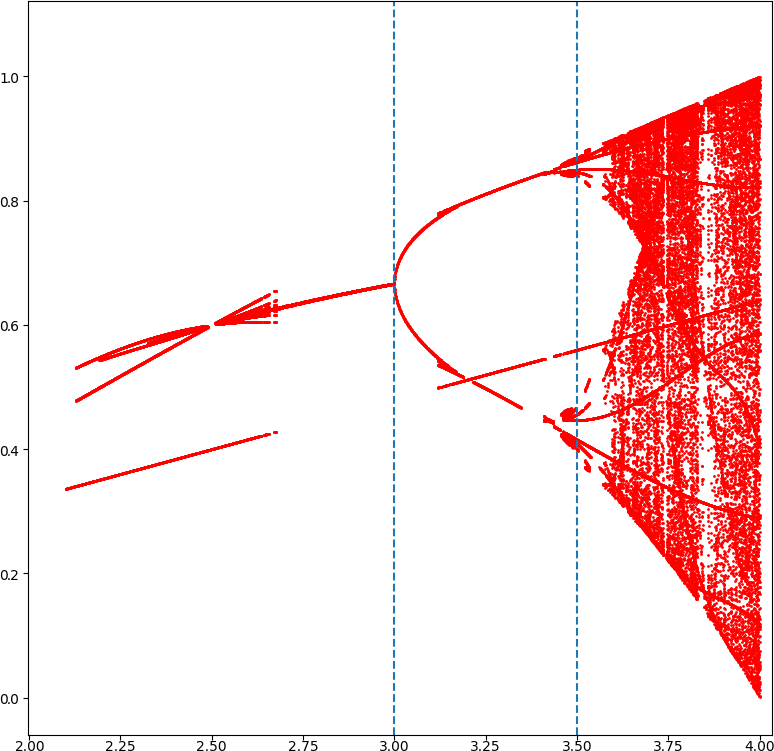
\includegraphics[width=0.5\linewidth]{fracaso}\\[5pt]
		{La primera gráfica que imprimí al empezar esta práctica.}
	\end{figure}
	
	\newpage
	
	\section{Introducción}
	En esta práctica analizamos la convergencia de un sistema dinámico no lineal. En este caso, la transformación asociada viene dada por la función logística: $f_r(x) = r\cdot x\cdot(1-x)$.
	Se usa para representar el crecimiento de poblaciones cuando la capacidad del ambiente es limitada.
	
	Esta función es dependiente de un parámetro $r\in\mathbb{R}$, por lo que el sistema cambia de comportamiento al modificar este parámetro. Veremos cómo son las cuencas de atracción para algunos valores de $r$, y cuáles tienen un tamaño determinado.
	
	\section{Material usado y metodología}
	Vamos a tomar un margen de error de $\varepsilon=0.001$ para todos los apartados. Además, en general, tomaremos el estado inicial $x_0=0.200$. 
	Tomamos $N_0=200$ como nuestra máxima capacidad de cómputo; supondremos que más allá perdemos precisión por errores de la computadora. También consideramos periodos de, como máximo, $N=20$.
	
	Los cálculos se realizarán en un \textit{script} de Python, adjuntado en la sección \ref{codigo}.
	
	\subsection{Apartado \textit{i})}
	
	En primer lugar, tomaremos dos valores del parámetro $r$ en $(3,3.544)$. Para cada uno, calculamos la órbita de ese sistema (hasta el término $N_0$), aplicando la función logística iterativamente. 
	
	Después, calculamos hasta qué paso de iteración \textemdash o tiempo transcurrido\textemdash~la órbita empieza a mantenerse estable. Nos quedaremos con la subórbita de tamaño $N$ a partir de $m\in\mathbb{N}$ tal que su diámetro y el de la subórbita siguiente no difieren de más de $\varepsilon$. Es decir, si $D(S)=\max(S)-\min(S)$:
	\[ \left|D\left(\{f_r^i(x_0)\}_{i=m-N}^{m}\right) - D\left(\{f_r^i(x_0)\}_{i=m}^{m+N}\right)\right| < \varepsilon \]
	
	Calculamos su conjunto atractor. Buscamos el periodo de la órbita: el primer $1<p\in\mathbb{N}$ tal que:	
	\[ \left|f_r^{m-1}(x_0) - f_r^{m-p}(x_0)\right| < \varepsilon \]
	
	El conjunto atractor serán los $p$ últimos valores de la subórbita calculada hasta el paso $m$.
	
	Calcularemos el intervalo de error del valor de la $r$ tomando valores cercanos a los escogidos y asegurándonos de que el conjunto atractor permanece estable. Es decir, si el conjunto atractor es $V_r(x_0)$, encontraremos un $\delta>0$ tal que, para $0<d<\delta$,
	\( \left| V_r(x_0) - V_{r\pm d}(x_0) \right|_\infty < \varepsilon \).
	
	Además veremos si cambiando el estado inicial $x_0$ también permanece estable. Encontraremos un $\delta>0$ para el que, si $0<d<\delta$,
	\( \left| V_r(x_0) - V_r(x_0\pm d) \right|_\infty < \varepsilon \).
	
	\subsection{Apartado \textit{ii})}
		
	En segundo lugar, buscamos los valores de $r$ tales que su cuenca de atracción es igual a 8.
	
	Para ello, calculamos para cada valor $r\in(3.544,4)$ \textemdash tomándolos de $\varepsilon$ en $\varepsilon$\textemdash~su conjunto de atracción, y comprobamos si su tamaño es 8. 
	
	Si lo es, comprobamos que al cambiar el estado inicial $x_0\pm\varepsilon$ el conjunto atractor sigue siendo el mismo.
	
%	datos que nos den, plantilla, escrito en ingles a codificar, etc
%	conjunto de condiciones iniciales parametros etc
%	datos de entrada
%	set de datos
%	condiciones
%	contorno espaciales temporales espaciales fijados
	
	
%	implementacion del sistema din no lineal mediante iteraciones y deteccion de cotas de error explicar calcular cota de error tomando conjunto de datos candidatos a la cuenca de atraccion menos la cuenca anterior, poner formulita
	
	\section{Resultados y conclusiones}
	\subsection{Apartado \textit{i})}
	
	Tomaremos $r=3.141$ y $r=3.515$.
	
	Para $r=3.141\pm 0.003$, el conjunto atractor calculado es $[0.538, 0.781]\pm \varepsilon$. Ha usado $m=60$ pasos para que el error cometido estuviera en el margen dado.
	Hemos calculado que, para $\delta=0.003$, $r+\delta$ da un conjunto atractor de [0.536, 0.782] $\pm \varepsilon$.
	
	Para $r=3.515\pm 0.002$, el conjunto atractor calculado es $[0.375, 0.509, 0.824, 0.878] \pm \varepsilon$. Ha usado $m=20$ pasos, muchos menos que para el valor anterior.
	Hemos calculado que, para $\delta=0.002$, $r+\delta$ da un conjunto atractor de $[0.374, 0.511, 0.824, 0.879] \pm \varepsilon$.
	
	En ambos casos, la elección de estado inicial $x_0\in(0,1)$ es irrelevante, ya que es suficientemente estable. También hemos comprobado que el mayor $r$ tiene un intervalo de error $\pm\delta$ menor. Por tanto, el conjunto atractor se ve modificado más rápidamente. 
	
	Entre ambos puntos escogidos hay al menos un punto de bifurcación, ya que el tamaño de la primera cuenca es 2 y la segunda es de 4.
	
	\subsection{Apartado \textit{ii})}%\vspace*{-2\bigskipamount}
	\begin{sidefig}{0.5}
	
	Hemos calculado, para $r\in(3.544,3.563)\pm \varepsilon$, que todas sus cuencas de atracción tienen 8 elementos. Además, hemos comprobado que con $x_0=0.200\pm \varepsilon$ sus cuencas de atracción se mantienen estables.\\[\medskipamount]
	Por ejemplo, para $r=3.550\pm \varepsilon$ se tiene el conjunto $[0.355, 0.370, 0.506, 0.540,0.813, 0.828, $ $0.882, 0.887]$ $\pm \varepsilon$. A la derecha se encuentra la gráfica de cada conjunto identificado en función de su $r$.\\[\medskipamount]
	A partir de $r=3.565\pm \varepsilon$ el conjunto de atracción ya no tiene 8 elementos sino 16, por lo que ha habido un punto de bifurcación en $3.564\pm\varepsilon$. Después, no volvemos a encontrar valores de $r$ con cuencas de atracción de tamaño 8.\\[\medskipamount]
	La bifurcación previa debe estar antes del valor $r=3.544$, ya que en el apartado $i)$ encontramos un conjunto de 4 elementos para $r=3.515$, así que debe haber alguna bifurcación entre ambos.
	
	\herefig{0.45}
	
	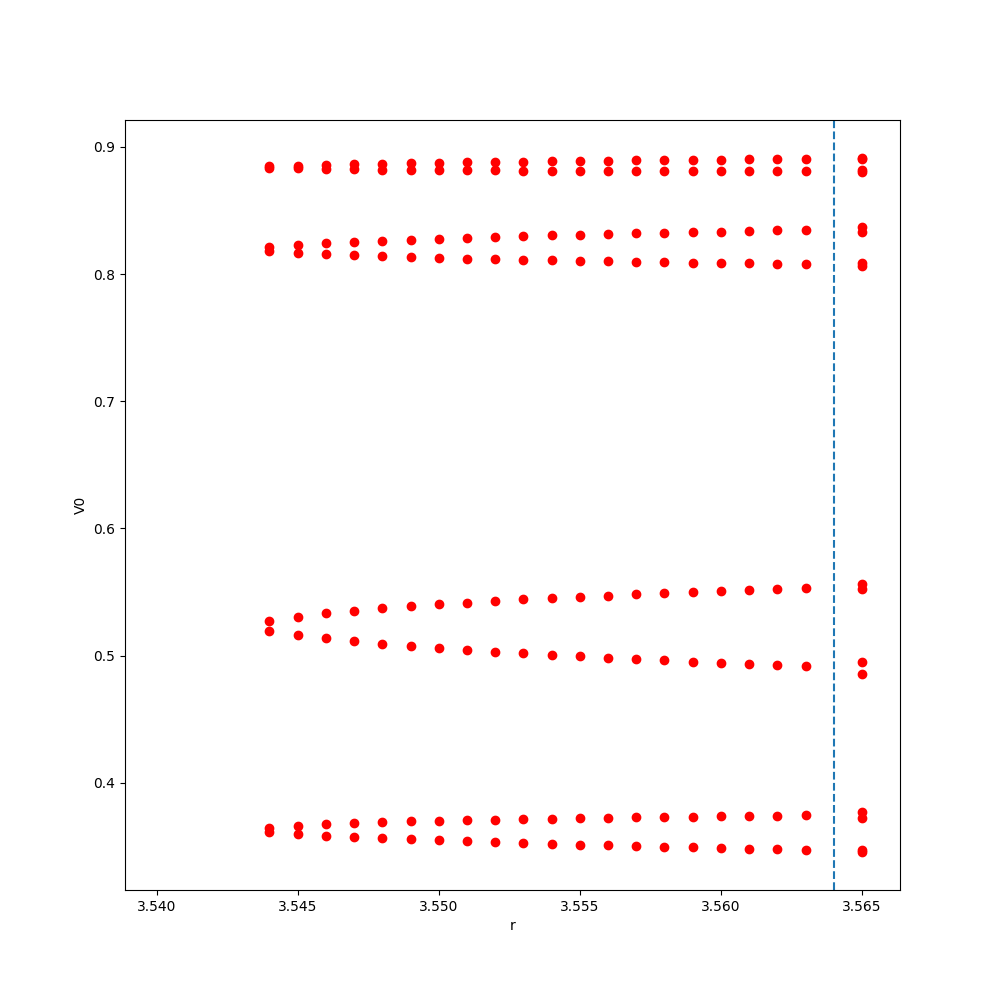
\includegraphics[width=\linewidth]{grafica}
	
	\end{sidefig}\vspace*{\smallskipamount}

	Con este experimento hemos analizado cómo se comporta el sistema dinámico logístico para algunos valores de su parámetro $r$. Hemos visto algunas de sus características en los intervalos de $(3.1,3.544)$ y $(3.544,4)$, calculando sus conjuntos atractores y midiendo las cotas de error en nuestros cálculos.

%	datos e interpretacion.
%	para r=3,2 obtenfo esto, para tal obtengo cual
%	
%	interpretable. obtengo que los tiempos de transicicon eran pequeños en comparacion con la computacion... que la estimacion de cota claramente es muy inferior a la diferencia de puntos que estoy obteniendo
	
%	\section{Conclusiones}
	
%	conclusiones (lo mismo...) no hace falta 10 apartados, pero el contenido tiene que estar
%	
%	graficas visuales. cuantas? el 50 como maximo
%	
%	criterios graficas vectoriales. memoria en latex jeje si pesan mucho esta bien, si tiene mala resolucion pero se ve no pasa nada
%	
%	el indice no cuenta, anexos tampoco. uno del codigo. y adjuntar el codigo independiente.	
%	
%	unir apartados segun sea necesario
%	por ej metodos y datos

	\newpage
	\section{Código}\label{codigo}
	
	\lstinputlisting[language=Python]{p1_rubiomadrigalcelia.py}
	
\end{document}